\documentclass[12pt, a4paper, oneside]{article}

\usepackage[utf8]{inputenc}
\usepackage{tikz}

\usepackage{listings}


\usepackage[
a4paper,
textwidth=175mm,
textheight=225mm,
heightrounded,
]{geometry}

\usepackage[T1]{fontenc} % <-- don't forget
\usepackage[utf8]{inputenc}
\usepackage[dutch]{babel}
\usepackage{graphicx}
\usepackage{pgfplots}
\usepackage[
backend=biber,
style=alphabetic,
sorting=ynt,
]{biblatex}
\addbibresource{references.bib}

\usepackage[hidelinks]{hyperref}

\usepackage[
a4paper,
textwidth=175mm,
textheight=225mm,
heightrounded,
]{geometry}

\usepackage[T1]{fontenc} % <-- don't forget
\usepackage[utf8]{inputenc}
\usepackage[dutch]{babel}
\usepackage{graphicx}
\usepackage{pgfplots}
\usepackage[
backend=biber,
style=alphabetic,
sorting=ynt,
]{biblatex}
\addbibresource{references.bib}

\usepackage[hidelinks]{hyperref}

\setlength{\parskip}{1.2ex}    % space between paragraphs
\setlength{\parindent}{0cm}%2em}       % amount of indention

\title{Hausaufgabe 3}
\author{Aaron Sastry}

\begin{document}

\maketitle

\textbf{Aufgabe 3.2 Heaps}
\begin{description}
	\item[a)] Fügen Sie die Werte 10, 4, 3, 15, 21, 2, 8, 11 und 1 in einen anfangs leeren Heap ein.
	Stellen Sie nach jeder Einfüge-Operation den Heap als Baum dar und geben Sie das Array an, welches dem fertigen Heap entspricht.
	\\
	
	\emph{insert: 10}
	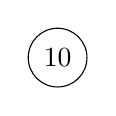
\begin{tikzpicture}
		\node[circle,draw](z){$10$};
	\end{tikzpicture}
	\emph{insert: 4}
	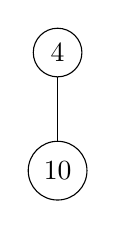
\begin{tikzpicture}
		\node[circle,draw](z){$4$}
		child{
			node[circle,draw]{10}};
	\end{tikzpicture}
	\emph{insert: 3}
	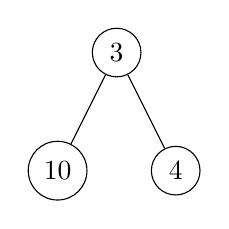
\begin{tikzpicture}
		\node[circle,draw](z){$3$}
		child{ node[circle,draw]{10}}
		child{node[circle,draw]{4}};
	\end{tikzpicture}
	
	\emph{insert: 15}
	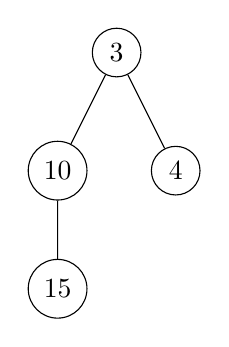
\begin{tikzpicture}
		\node[circle,draw](z){$3$}
		child{
			node[circle,draw]{10}  child{node[circle,draw]{15}}}
		child{node[circle,draw]{4}};
	\end{tikzpicture}
	\emph{insert: 21}
	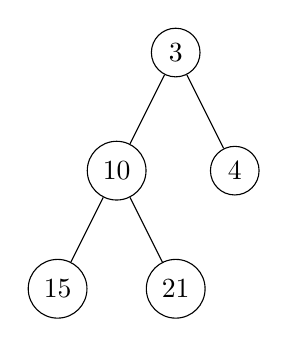
\begin{tikzpicture}
		\node[circle,draw](z){$3$}
		child{
			node[circle,draw]{10}  child{node[circle,draw]{15}} child{node[circle,draw]{21}}}
		child{node[circle,draw]{4}};
	\end{tikzpicture}\\
	\emph{insert: 2}
	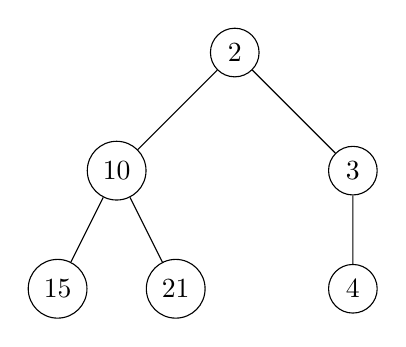
\begin{tikzpicture}[level distance=1.5cm,
		level 1/.style={sibling distance=3cm},
		level 2/.style={sibling distance=1.5cm}]
		\node[circle,draw](z){$2$}
		child{
			node[circle,draw]{10}  
			child{node[circle,draw]{15}} 
			child{node[circle,draw]{21}}}
		child{
			node[circle,draw]{3} 
			child{node[circle,draw]{4}}};
	\end{tikzpicture}
	\emph{insert: 8}
	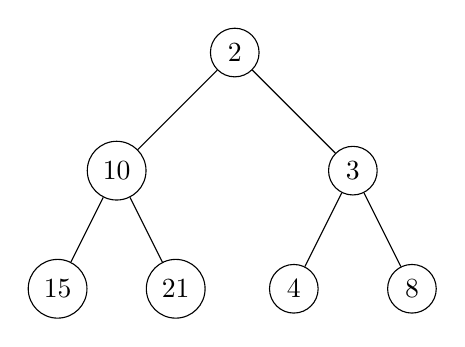
\begin{tikzpicture}[level distance=1.5cm,
		level 1/.style={sibling distance=3cm},
		level 2/.style={sibling distance=1.5cm}]
		\node[circle,draw](z){$2$}
		child{
			node[circle,draw]{10}  
			child{node[circle,draw]{15}} 
			child{node[circle,draw]{21}}}
		child{
			node[circle,draw]{3} 
			child{node[circle,draw]{4}} 
			child{node[circle,draw]{8}}};
	\end{tikzpicture}\\
	\emph{insert: 11}
	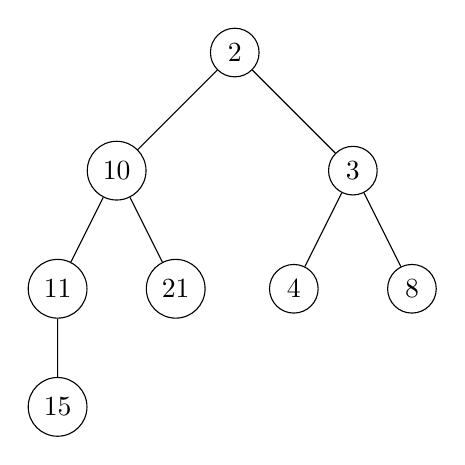
\begin{tikzpicture}[level distance=1.5cm,
		level 1/.style={sibling distance=3cm},
		level 2/.style={sibling distance=1.5cm}]
		\node[circle,draw](z){$2$}
		child{
			node[circle,draw]{10}  
			child{node[circle,draw]{11}
				child{node[circle,draw]{15}}} 
			child{node[circle,draw]{21}}}
		child{
			node[circle,draw]{3} 
			child{node[circle,draw]{4}} 
			child{node[circle,draw]{8}}};
	\end{tikzpicture}
	\emph{insert: 1}
	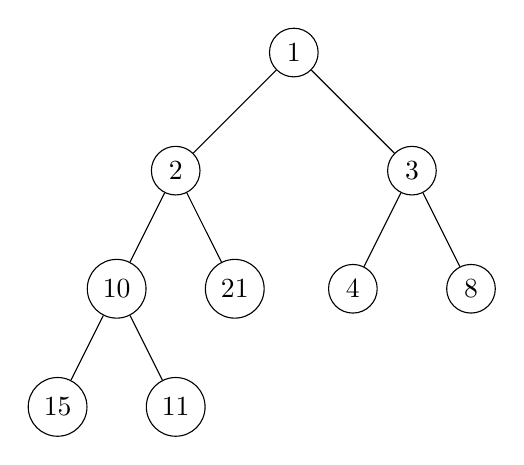
\begin{tikzpicture}[level distance=1.5cm,
		level 1/.style={sibling distance=3cm},
		level 2/.style={sibling distance=1.5cm}]
		\node[circle,draw](z){$1$}
		child{
			node[circle,draw]{2}  
			child{node[circle,draw]{10}
				child{node[circle,draw]{15}}
				child{node[circle,draw]{11}}} 
			child{node[circle,draw]{21}}}
		child{
			node[circle,draw]{3} 
			child{node[circle,draw]{4}} 
			child{node[circle,draw]{8}}};
	\end{tikzpicture}
	
	Das array zu diesem heap sieht wie folgt aus:\\
	\emph{heap = [1, 2, 3, 10, 21, 4, 8, 15, 11]}
	\newline
	
	
	\item[b)] Führen Sie auf dem soeben gebauten Heap zwei deleteMin-Operationen durch und
	geben Sie jeweils den resultierenden Heap in Baumdarstellung und als Array an.
	
	Lösche das Min-Element:\\
	\emph{deleteMin}
	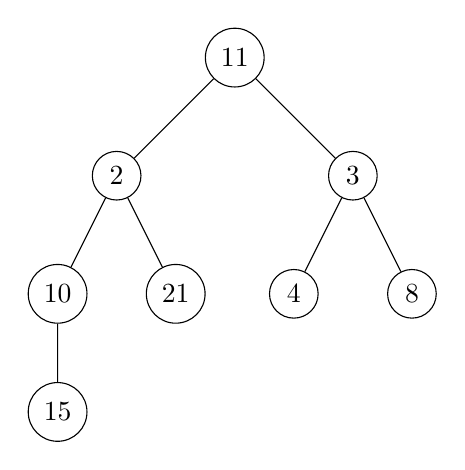
\begin{tikzpicture}[level distance=1.5cm,
		level 1/.style={sibling distance=3cm},
		level 2/.style={sibling distance=1.5cm}]
		\node[circle,draw](z){$11$}
		child{
			node[circle,draw]{2}  
			child{node[circle,draw]{10}
				child{node[circle,draw]{15}}} 
			child{node[circle,draw]{21}}}
		child{
			node[circle,draw]{3} 
			child{node[circle,draw]{4}} 
			child{node[circle,draw]{8}}};
	\end{tikzpicture}
	\emph{siftDown}
	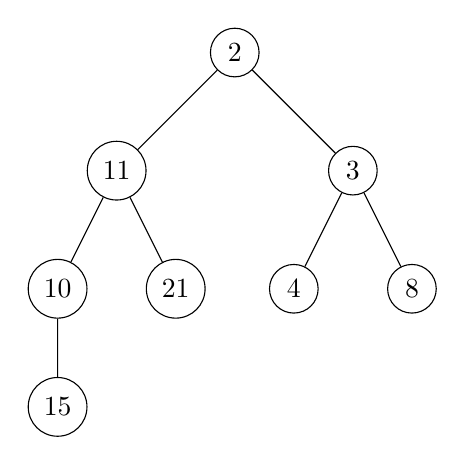
\begin{tikzpicture}[level distance=1.5cm,
		level 1/.style={sibling distance=3cm},
		level 2/.style={sibling distance=1.5cm}]
		\node[circle,draw](z){$2$}
		child{
			node[circle,draw]{11}  
			child{node[circle,draw]{10}
				child{node[circle,draw]{15}}} 
			child{node[circle,draw]{21}}}
		child{
			node[circle,draw]{3} 
			child{node[circle,draw]{4}} 
			child{node[circle,draw]{8}}};
	\end{tikzpicture}
	\emph{siftDown}
	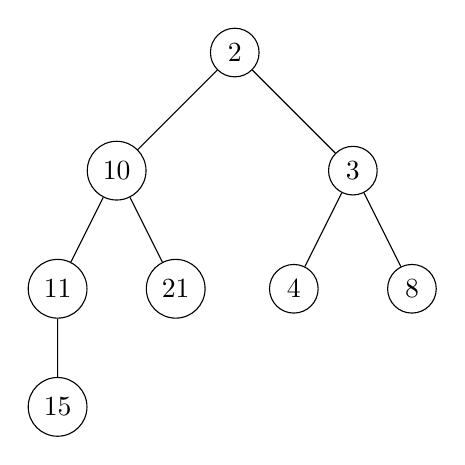
\begin{tikzpicture}[level distance=1.5cm,
		level 1/.style={sibling distance=3cm},
		level 2/.style={sibling distance=1.5cm}]
		\node[circle,draw](z){$2$}
		child{
			node[circle,draw]{10}  
			child{node[circle,draw]{11}
				child{node[circle,draw]{15}}} 
			child{node[circle,draw]{21}}}
		child{
			node[circle,draw]{3} 
			child{node[circle,draw]{4}} 
			child{node[circle,draw]{8}}};
	\end{tikzpicture}
	
	Min-Element gelöscht\\
	output: \emph{deleted element is 1}\\	
	Neues Min-Element ist: \emph{2}\\
	der heap sieht nun wie folgt aus: \emph{[2, 10, 3, 11, 21, 4, 8, 15]}\\
	
	Lösche nun das nächste Min-Element:\\
	\emph{deleteMin}
	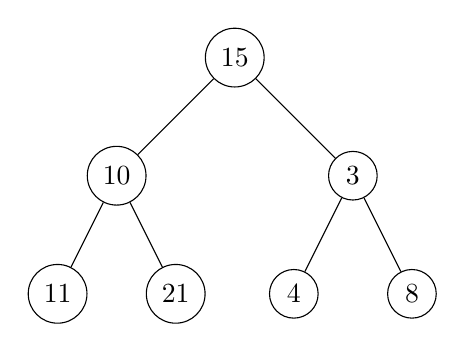
\begin{tikzpicture}[level distance=1.5cm,
		level 1/.style={sibling distance=3cm},
		level 2/.style={sibling distance=1.5cm}]
		\node[circle,draw](z){$15$}
		child{
			node[circle,draw]{10}  
			child{node[circle,draw]{11}} 
			child{node[circle,draw]{21}}}
		child{
			node[circle,draw]{3} 
			child{node[circle,draw]{4}} 
			child{node[circle,draw]{8}}};
	\end{tikzpicture}
	\emph{siftDown}
	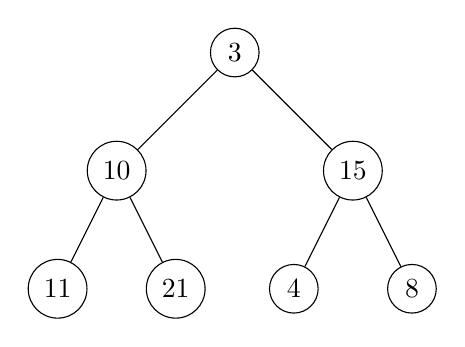
\begin{tikzpicture}[level distance=1.5cm,
		level 1/.style={sibling distance=3cm},
		level 2/.style={sibling distance=1.5cm}]
		\node[circle,draw](z){$3$}
		child{
			node[circle,draw]{10}  
			child{node[circle,draw]{11}} 
			child{node[circle,draw]{21}}}
		child{
			node[circle,draw]{15} 
			child{node[circle,draw]{4}} 
			child{node[circle,draw]{8}}};
	\end{tikzpicture}
	\emph{siftDown}
	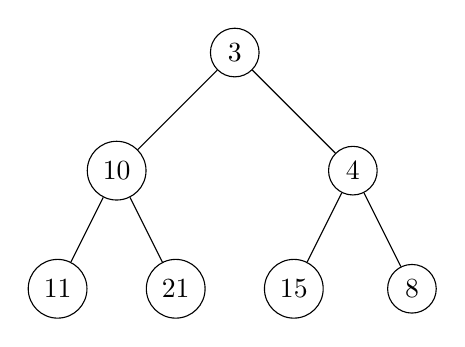
\begin{tikzpicture}[level distance=1.5cm,
		level 1/.style={sibling distance=3cm},
		level 2/.style={sibling distance=1.5cm}]
		\node[circle,draw](z){$3$}
		child{
			node[circle,draw]{10}  
			child{node[circle,draw]{11}} 
			child{node[circle,draw]{21}}}
		child{
			node[circle,draw]{4} 
			child{node[circle,draw]{15}} 
			child{node[circle,draw]{8}}};
	\end{tikzpicture}
	
	Min-Element gelöscht\\
	output: \emph{deleted element is 2}\\	
	Neues Min-Element ist: \emph{3}\\
	der heap sieht nun wie folgt aus: \emph{[3, 10, 4, 11, 21, 15, 8]}\\
	\newline
	\\
	
	\item[c)] Beschreiben Sie einen Algorithmus, der k sortierte Listen mit Gesamtlänge n in
	O(n log k) Zeit zu einer sortierten Liste zusammenfügt. Benutzen Sie dabei einen Heap.
	Begründen Sie kurz, dass Ihr Algorithmus die Laufzeitschranke einhält.\\
	\newline
	
	\begin{lstlisting}
		
	sortListwithHeap(A: Array of k lists)
			
		sei B ein leerer heap
			
		sei C ein leeres array
		sei D ein leeres array
			
		for i <- 1 to k do
			
			/*tupel aus der value des minElemets 
			der list und der listenNummer */
			C.append([A[i][1], k])
			
			Remove(A[i][1])
			
		B.BuildMinHeap(C)
							
		for i <- 1 to n do
		    item = B.minElement
		    listnumber = item[2]
		    deleteMin()
		    D.append(item[1])
				
		    if A[listnumber] nicht leer
		        B.insert((A[listnumber][1], listnumber))
		        Remove(A[listnumber][1])
				
			
	\end{lstlisting}

	Dieser Algorythmus hält die schranke ein, da deleteMin() und insert() laut VL in O(log(n)) sind, und dies wird n mal getan $\rightarrow$ O(n log(n))
	
	\item[d)] Gegeben sei die folgende alternative Prozedur zum Erstellen eines binären Heaps für
	ein unsortiertes Array A[1..n]:
	\begin{lstlisting}
		buildHeapInsert(A : Array):
		 	for i <- 1 to n do
		 	insert(A[i])
	\end{lstlisting}
	Geben Sie ein Beispiel für eine Eingabe an, sodass buildHeapInsert eine schlechtere
	Laufzeit für das Aufbauen des Heaps hat als O(n). Was ist die worst–case Laufzeit von
	buildHeapInsert? Begründen Sie!
	
	\textbf{Antwort:}\\
	Im schlechtesten Falle ist für jedes Element i, dass eingefügt wird das folgende i+1 Element, welches dannach eingefügt wird kleiner als i, sodass jedes Element immer per siftUp bis auf die Min-Position hoch gegeben werden muss.
	
	Somit würde Insert des i-ten Elements in \(\lfloor$log(i)$\rfloor\) passieren.
	Und der gesammt aufbau wäre in:
	
	\centerline{\(O(\sum^{n}_{i=1}log(i)) \Longleftrightarrow O(log(n!))\)}
	\centerline{   }
	
	Sobald nun log(i) > 1, wird auch die Summe \(\sum^{n}_{i=1}log(i)\) bald größer als die summe \(\sum^{n}_{i=1}1\) 
	
	\centerline{\(\Longrightarrow O(log(n!)) > O(n)\)}
	\centerline{Stirling's approximation}
	\centerline{\(\Longrightarrow O(log(n!)) = O(n log(n))\)}
	
	
\end{description}
	
\end{document}